\ifdefined\COMPLETE
\else
\documentclass[11pt]{article}
\usepackage[french, english]{babel}
\usepackage[utf8]{inputenc}
\usepackage{graphicx}
\usepackage{framed}
\usepackage[normalem]{ulem}
\usepackage{amsmath}
\usepackage{amsthm}
\usepackage{amssymb}
\usepackage{amsfonts}
\usepackage{enumerate}
\usepackage{import}
\usepackage[top=1 in,bottom=1in, left=1 in, right=1 in]{geometry}
\usepackage{listingsutf8}
\usepackage{color}
\usepackage{float}
\usepackage{graphicx}
\usepackage{subcaption}
\usepackage[toc,page]{appendix}
\usepackage{multicol}
\usepackage{wrapfig}
\usepackage{sidecap}

\floatstyle{boxed} 
\restylefloat{figure}
\definecolor{mygreen}{rgb}{0,0.6,0}
\definecolor{mygray}{rgb}{0.5,0.5,0.5}
\definecolor{mymauve}{rgb}{0.58,0,0.82}
\newcommand{\dt}{\partial_t}
\newcommand{\Tl}{\frac{T}{\lambda}}
\theoremstyle{definition}
\newtheorem{definition}{Définition}[section]
\DeclareMathOperator*{\argmax}{arg\,max}
\DeclareMathOperator*{\argmin}{arg\,min}
 


\lstset{ 
  backgroundcolor=\color{white},   % choose the background color; you must add \usepackage{color} or \usepackage{xcolor}; should come as last argument
  basicstyle=\footnotesize,        % the size of the fonts that are used for the code
  breakatwhitespace=false,         % sets if automatic breaks should only happen at whitespace
  breaklines=true,                 % sets automatic line breaking
  captionpos=b,                    % sets the caption-position to bottom
  commentstyle=\color{mygreen},    % comment style
  deletekeywords={...},            % if you want to delete keywords from the given language
  escapeinside={\%*}{*)},          % if you want to add LaTeX within your code
  extendedchars=true,              % lets you use non-ASCII characters; for 8-bits encodings only, does not work with UTF-8
  firstnumber=1000,                % start line enumeration with line 1000
  frame=single,	                   % adds a frame around the code
  keepspaces=true,                 % keeps spaces in text, useful for keeping indentation of code (possibly needs columns=flexible)
  keywordstyle=\color{blue},       % keyword style
  language=Python,                 % the language of the code
  morekeywords={*,...},            % if you want to add more keywords to the set
  numbers=left,                    % where to put the line-numbers; possible values are (none, left, right)
  numbersep=5pt,                   % how far the line-numbers are from the code
  numberstyle=\tiny\color{mygray}, % the style that is used for the line-numbers
  rulecolor=\color{black},         % if not set, the frame-color may be changed on line-breaks within not-black text (e.g. comments (green here))
  showspaces=false,                % show spaces everywhere adding particular underscores; it overrides 'showstringspaces'
  showstringspaces=false,          % underline spaces within strings only
  showtabs=false,                  % show tabs within strings adding particular underscores
  stepnumber=2,                    % the step between two line-numbers. If it's 1, each line will be numbered
  stringstyle=\color{mymauve},     % string literal style
  tabsize=2,	                   % sets default tabsize to 2 spaces
  title=\lstname                   % show the filename of files included with \lstinputlisting; also try caption instead of title
}
\lstset{inputencoding=utf8/latin1}
\newcommand{\Dt}{\Delta t}
\newcommand{\Dx}{\Delta x}
 %file containing all the used libraries
\newtheorem{theorem}{Théorème}
\begin{document}
\fi
\section{Recherche de la vitesse d'onde des solutions progressives de l'Équation fluide complète du champignon.}
Le but de cette section est de montrer comment l'on peut obtenir la vitesse d’onde pour l’équation du champignon complète:  
\begin{equation}  \left\{
                \begin{array}{ll}
                \dt\mu + \nabla(\mu v) = f(C)(\mu + \rho) -\mu\rho \\
                   \dt(\mu v)+\nabla(\mu v\times v) +T\nabla\mu=-\lambda\mu v+\mu\nabla C-\mu v \rho \\
                 \dt\rho=  F(v) \mu \\
                  \dt C = -b\rho C.
                \end{array}
              \right.
\end{equation} 
En effet dans les sections précédentes nous avons travaillés dans le cas $\lambda$ et $T$ très grands ce qui simplifiait les équations.\\
Cependant nous avons pu voir que, comme pour l’équation de Fisher KPP, pour une donnée initiale à support compact, la solution tend vers une solution d'onde et que la vitesse d'onde peut être retrouvée grâce a la linéarisation autour de l'état initial.\\
Nous allons alors adopter la même stratégie pour l’équation complète.\\
Ici nous allons linéariser autour de l’état $(\mu,\rho,C,v) = (0,0,C_0,v)$.\\
Équation d'onde pour le fluide:\\
Soit $s$ la vitesse d'onde, $y=x-st$, par le même argument de symétrie que pour l’équation de  ``KPP avec mémoire", nous allons se placer dans le cas $s<0$. Avec abus de notation $ :(x,t) = :(y)$, où $y=x-st$, l’équation d'onde pour le fluide est:
\begin{equation}\label{eq:FWS_BDNG}  \left\{
                \begin{array}{ll}
                -s\mu' + (\mu v)' = f(C)(\mu + \rho) -\mu\rho \\
                   -s (\mu v)'+(\mu v\times v)' +T\mu'=-\lambda\mu v+\mu C'-\mu v \rho \\
                 -s \rho '=  F(v) \mu \\
                  -sC' = -b\rho C.
                \end{array}
              \right.
\end{equation} 
Linéarisation autour de l’état  $(\mu,\rho,C,v) = (0,0,C_0,v)$: \\
On pose $f(C_0) = f_0$, et on cherche des solutions de la forme $\rho = \rho_0 \exp(Xy)$ autour de $\rho=0$.\\ 
On obtient en intégrant la quatrième ligne $C= C_0 - \frac{b\rho_0 C_0}{X}\exp(Xy).$\\
La troisième ligne donne: $-sX\rho_0\exp(Xy)=F_0\mu$ donc $\mu = \frac{-sX\rho_0}{F_0}\exp(Xy)$.\\
Autour de $(\mu,\rho,C,v) = (0,0,C_0,v)$, la première ligne donne: $-s\mu' + (\mu v)' = f_0(\mu + \rho)$ car on peut négliger $\mu\rho$ devant $\mu$ et $\rho$ . On a donc \begin{equation}
	(\mu v)'=(f_0\rho_0-\frac{sXf_0\rho_0}{F_0}-\frac{s^2X^2\rho_0}{F_0})\exp(Xy)
\end{equation}
donc \begin{equation}
	\mu v = (\frac{f_0\rho_0}{X}- \frac{f_0s\rho_0}{F_0}-\frac{s^2X\rho_0}{F_0})\exp(Xy).
\end{equation}
Ainsi \begin{equation}
	v= \frac{\mu v}{\mu} = v_0 = s + \frac{f_0}{X}-\frac{f_0F_0}{X^2s}  .
\end{equation}
La deuxième ligne donne $-s (\mu v)'+(\mu v\times v)' +T\mu'=-\lambda\mu v+\mu C'-\mu v \rho$. \\
On peut ici négliger $\mu v\rho$ et $\mu C'$ devant $\mu v$. On a donc: \begin{equation}
	(-v_0sX\mu_0 + v_0^2X\mu_0 +T\mu_0X)\exp(Xy) = -\lambda\mu_0v_0\exp(Xy)
\end{equation}
donc \begin{equation}
	-sXv_0 + v_0^2X+ TX = -\lambda v_0.
\end{equation}
En multipliant par $X^2$ et en substituant $v_0 =  s + \frac{f_0}{X}-\frac{f_0F_0}{X^2s}$ on a alors l’équation caractéristique:
\begin{equation} \label{eq:P}
	X^4(Ts^2) + X^3(\lambda + f_0)s^3+ X^2(f_0^2s^2+ \lambda f_0 s^2 - f_0F_0s^2)+ X(-sF_0f_0)(\lambda+2f_0) + f_0^2F_0^2=0.
\end{equation}
En posant $Y = sX$ on obtient: \begin{equation}
	A(Y) \equiv Y^4+\frac{s^2}{T}P_3(Y)=0 \label{eq:PY}
\end{equation} où \begin{equation}
		P_3(Y) \equiv  Y^3(\lambda + f_0)+ Y^2(f_0^2+ \lambda f_0 - f_0F_0)- Y(F_0f_0(\lambda+2f_0)) + f_0^2F_0^2
\end{equation} est un polynôme de degré 3 dont les coefficients ne dépendent que des données $f_0$, $F_0$, $\lambda$ et $T$. \\
\subsection{Condition d'existence de racines toutes réelles}
La vitesse recherchée est le plus petit $s>0$ (ou plus grand $s<0$ ) tel que le polynôme de degré 4 $A$ défini dans \ref{eq:PY} possède quatre racines réelles (comptées avec multiplicité).\\ 
Effectuons le changement de variable $Y= Y-\frac{b}{4}$ où $b$ est le coefficient devant $Y^3$ dans $A$ et posons $S= \frac{s^2}{T}>0$.\\
 Ce nouveau polynôme (noté $B$) s'écrit: \begin{equation}
	B(Y) \equiv A(Y-\frac{b}{4}) = Y^4 + qY^2 + r Y + \sigma.
\end{equation}
$B$ est dénommé le polynôme réduit de $A$ : on a annulé le terme en $Y^3$.
Pour que $B$ ait 4 racines réelles, les coefficients de $B$ doivent satisfaire trois conditions (de façon nécessaire et suffisante) CITER EQUATION D'ORDRE 4:\\
i) $q<0$,\\
ii) $q^2-4\sigma>0$,\\
iii) Le discriminant $\Delta_B$ de $B$ est positif: $\Delta_B>0$.\\
Les calculs étant très lourds, j'ai utilisé un module de calcul formel pour les effectuer et trouver des factorisations et simplifications. Dans toute la suite, comme $S= \frac{s^2}{T}$, on s’intéressera aux conditions dans le cas $S>0$.
\subsubsection{Condition $q<0$}
On a \begin{equation} q = - \frac{S \left( S \left(3 \lambda^{2} + 6 \lambda f_{0} + 3 f_{0}^{2}\right)+ 8 F_{0} f_{0} + - 8 \lambda f_{0} - 8 f_{0}^{2}\right)}{8}. \end{equation}
Ainsi on a $q<0$ sur un domaine de la forme $[a,\infty[$. Ce domaine est illustré dans la sous-section récapitulative suivante.

\newpage
\subsubsection{Condition $q^2 -4\sigma>0$}
Le calcul formel donne:
\begin{multline}
 q^2 - 4\sigma= S^{3}  \left( \frac{3  \lambda^{4}}{16} +  \frac{3  \lambda^{3} f_{0}}{4} +  \frac{9  \lambda^{2} f_{0}^{2}}{8} +  \frac{3  \lambda f_{0}^{3}}{4} +  \frac{3 f_{0}^{4}}{16} \right) \\ + S^{2}  \left(F_{0}  \lambda^{2} f_{0} + 2 F_{0}  \lambda f_{0}^{2} + F_{0} f_{0}^{3} -  \lambda^{3} f_{0} - 3  \lambda^{2} f_{0}^{2} - 3  \lambda f_{0}^{3} - f_{0}^{4} \right) \\+ S  \left(F_{0}^{2} f_{0}^{2} - F_{0}  \lambda^{2} f_{0} - 5 F_{0}  \lambda f_{0}^{2} - 4 F_{0} f_{0}^{3} +  \lambda^{2} f_{0}^{2} + 2  \lambda f_{0}^{3} + f_{0}^{4} \right)- 4 F_{0}^{2} f_{0}^{2} .
\end{multline}
En particulier c'est un polynôme de degré 3, de coefficient dominant positif, et négatif en $0$.\\ Il admet donc une ou trois racines strictement positives. \\ Dans le premier cas, on a $q^2 -4\sigma>0$ sur un domaine de la forme $[b,\infty[$ et dans le deuxième cas $[b,c[\cup [d,+\infty[ $. Ces cas et ces domaines sont illustrés dans la sous-section récapitulative suivante.


\subsubsection{Condition $\Delta_B >0$}
Le calcul formel montre que $\Delta_B$ s’écrit de la forme: \begin{equation}
	\Delta_B = S^3 L(S)
\end{equation}
où $L$ est un polynôme de degré au plus 3 en $S$. \\
Plus particulièrement:\\
- Son coefficient en $S^3 $ est égal à: \begin{equation}
	F_{0}^{2} f_{0}^{3} \left(4 F_{0} + f_{0} \right)  \left( \lambda + f_{0} \right)^{2}  \left(F_{0} f_{0} -  \lambda^{2} -  \lambda f_{0} \right)^{2} \geq 0
\end{equation} 
- Son discriminant $\Delta_L$ est égal à: \begin{multline} \Delta_L =16 F_{0}^{12} \lambda^{2} f_{0}^{15} \left(4 F_{0} f_{0} - \lambda^{2} - 2 \lambda f_{0}\right)^{2}\\ (32 F_{0}^{3} f_{0}^{2} + 9 F_{0}^{2} \lambda^{2} f_{0} + 48 F_{0}^{2} \lambda f_{0}^{2} + 48 F_{0}^{2} f_{0}^{3} + 27 F_{0} \lambda^{4} + 63 F_{0} \lambda^{3} f_{0} + 60 F_{0} \lambda^{2} f_{0}^{2} + 48 F_{0} \lambda f_{0}^{3} \\ + 24 F_{0} f_{0}^{4} + 9 \lambda^{4} f_{0} + 22 \lambda^{3} f_{0}^{2} + 21 \lambda^{2} f_{0}^{3} + 12 \lambda f_{0}^{4} + 4 f_{0}^{5})^{3} \geq 0 \end{multline}
Donc $\Delta_L \geq 0 $ et donc $L$ a trois racines.\\
- Son terme de degré nul $L(0)=256f_0^6F_0^6$ est positif: $L(0)>0$.\\
Ainsi $\Delta_B$ a zéro ou deux racines strictement positives, ce qui donne dans le premier cas un domaine de vitesse possible de la forme $[0,\infty[$ pour cette condition et dans le deuxième cas $[0,e[\cap[f,+\infty[.$ Ces cas et ces domaines sont illustrés dans la sous-section récapitulative suivante.
\subsubsection{Domaine des vitesses possibles et existence d'une vitesse minimale}
La deuxième condition montre en particulier l'existence d'une vitesse minimale strictement positive (en valeur absolue) de propagation. 
Le domaine du carré des vitesses possible étant l'intersection des trois domaines relatifs aux conditions, il est de la forme:
\begin{equation}
	\mathcal{D}=[a,b[\cap[c,d[\cap[e,+\infty[ \text{ ou } \mathcal{D}=[a,b[\cap[c,+\infty[ \text{ ou } \mathcal{D}=[a,+\infty[
\end{equation}
où $0<a<b<c<d<e$.\\
\newpage
\subsubsection{Récapitulatif et discussion graphique des trois conditions.}
Partout, la zone $S<0$ est invalide (rouge) car $S=\frac{s^2}{T}>0$.\\
Le domaine des vitesses possible est alors l'intersection des domaines valides (verts) pour les trois conditions:

i) Deux cas possibles sur la condition $q(S)<0$:\\


\begin{tabular}{cc}
 La racine de $q/S$ est positive & La racine de $q/S$ est négative \\
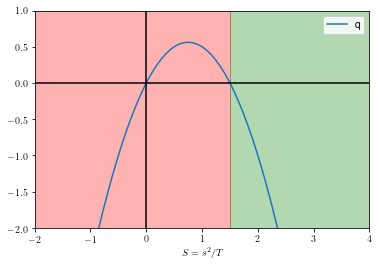
\includegraphics[width=.47\textwidth]{Images/qcas1.png} & 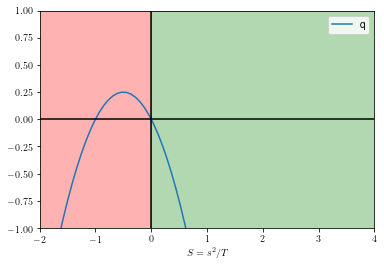
\includegraphics[width=.47\textwidth]{Images/qcas2.png} \\
\end{tabular}
\\
ii) Deux cas possibles sur la condition $q(S)^2-4\sigma(S)>0$:\\

\begin{tabular}{cc}
Une racine positive. & Trois racines positives. \\
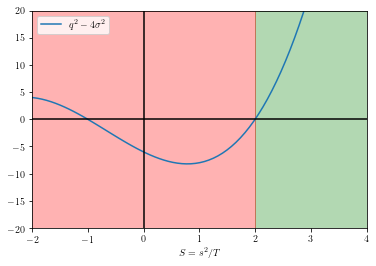
\includegraphics[width=.47\textwidth]{Images/q2cas1.png} & 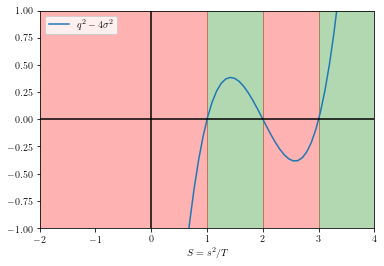
\includegraphics[width=.47\textwidth]{Images/q2cas2.png} \\
\end{tabular}
iii) Deux cas possibles sur la condition $\Delta_A(S) >0$:\\

\begin{tabular}{cc}
Trois racines négatives. & Une racine négative et deux positives.\\
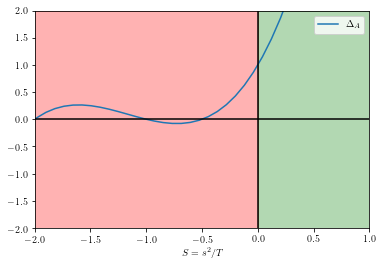
\includegraphics[width=.47\textwidth]{Images/deltacas1.png} & 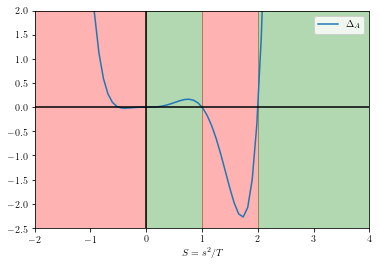
\includegraphics[width=.47\textwidth]{Images/deltacas2.png} \\
\end{tabular}






\subsection{Condition d'amortissement et détermination de la vitesse d'onde sélectionnée}
Lors des simulations, on s’aperçoit que la vitesse d'onde sélectionnée n'est pas pour tous les paramètres $\lambda,f_0,F_0,T$ le plus petit $s$ tel que le polynôme $A$ admet 4 racines réelles. Une autre condition apparaît: le $s$ cherché est la plus petite vitesse d'onde positive (ou la plus grande négative) tel que la linéarisation autour de l’état $(\mu,\rho,C,v) = (0,0,C_0,v_0)$ satisfait une condition dite "d'amortissement".
\begin{definition}{\textbf{Condition d'amortissement}} \\ Un polynôme $P \in \mathbb{R}[X]$ est dit satisfaire la condition d'amortissement pour notre problème si sa racine de plus petite partie réelle négative est réelle.
\end{definition}

La condition d'amortissement pour un polynôme montre que la dynamique de l'EDO liée au polynôme
\begin{theorem}\textbf{{Condition d'amortissement et positivité} }\\
$P$ vérifie la condition d'amortissement si et seulement si l'EDO associée à P ne s'annule pas autour de $-\infty$ pour des données initiales positives.
\end{theorem}
\begin{proof}Si $P$ vérifie la condition d'amortissement, soit alors $r_1$ la racine de plus petite partie réelle de $P$: elle est réelle. \\ 
Les solutions de l'EDO associé à $P$ avec conditions initiales positives sont de la forme: \begin{equation}
	f(x)=A_1\exp(r_1x)+ \sum_{i>1,r_i\in\mathbb{R}}(A_i\exp(r_ix)) + \sum_{i>1,r_i\not\in\mathbb{R}}B_i\exp(\Re(r_i))\cos(\omega_it)
\end{equation}
En particulier quand $x\to -\infty$, $f(x)\sim  A_1\exp(r_1x) >0$.\\
Réciproquement, les solutions $f$ de l'EDO sont équivalentes à $A_i\exp(\Re(r_i))cos(\omega_it)$, où $r_i$ est la racine de plus petite partie réelle. Pour ne pas avoir d’annulation, il faut $\omega_i =0 $ donc $r_i \in \mathbb{R}.$
\end{proof}


\subsubsection{Recherche de la vitesse d'onde extrémale satisfaisant la condition d'amortissement}
Soit $Y$ une racine du polynôme A défini \ref{eq:PY}, $s$ est déterminé par $Y$ par l'équation: \begin{equation}
	s^2 = -\frac{TY^4}{P_3(Y)}. \label{eq:sfromY}
\end{equation} 
Étudions alors la fonction $ s: Y \mapsto s(Y) = -\sqrt{\frac{TY^4}{P_3(Y)}} $.

\paragraph{Intervalle de définition:}
s(Y) est défini pour tous les $Y$ tels que $P_3(Y)<0$. Étudions alors le polynôme $P_3(Y)=Y^3(\lambda + f_0)+ Y^2(f_0^2+ \lambda f_0 - f_0F_0)- Y(F_0f_0(\lambda+2f_0)) + f_0^2F_0^2$:\\
i) Le coefficient dominant de $P_3$ est positif.\\
ii) Son discriminant est égal à: \begin{equation}
	\Delta_{P_3}= F_{0}^{2} f_{0}^{3} (4 F_{0} + f_{0}) (F_{0} f_{0} -\lambda ^{2} - \lambda  f_{0})^{2} \geq 0.
\end{equation}
Donc $P_3$ a 3 racines réelles (comptées avec multiplicité), notées $r_1\leq r_2 \leq r_3$.\\
iii) Le coefficient constant de $P_3$ est positif donc $-r_1r_2r_3>0$. Donc $r_1<0$, et $r_2$ et $r_3$ sont de même signe. Le coefficient d'ordre 1 de $P_3$ est négatif, donc $r_1r_2 + r_2r_3 + r_1r_3<0$ donc $r_1(r_2+r_3)+r_2r_3<0$ donc $r_2+r_3>0$ donc $r_2>0$ et $r_3>0$. $P_3$ a donc une racine négative et deux racines positives.

\begin{tabular}{cc}
 Polynôme $P_3(Y)$ & Fonction $s(Y) = -\sqrt{\frac{TY^4}{P_3(Y)}}$ \\
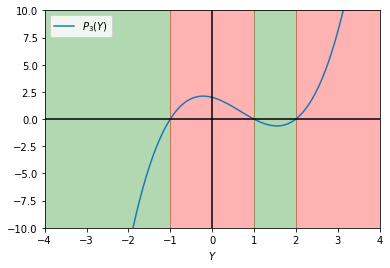
\includegraphics[width=.47\textwidth]{Images/P3.png} & 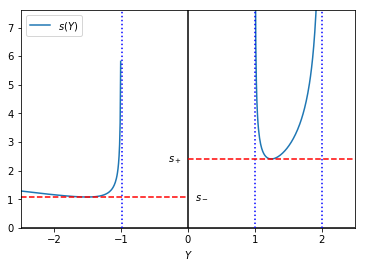
\includegraphics[width=.47\textwidth]{Images/s+s-.png} \\
\end{tabular}

\paragraph{Extremums:} Les extremums de $s$ sont définis par la relation:\begin{equation}
	\frac{\partial s}{\partial Y}=0
\end{equation}
Donc nécessairement: \begin{equation}
	\Big(\frac{Y^4}{P_3(Y)}\Big)'=0
\end{equation} 
i.e. \begin{equation}
\label{eq:Q}	Q(Y)\equiv4P_3(Y)-YP'_3(Y)=0
\end{equation}
Y est alors une racine du polynôme $Q$ défini ci dessus.\\
 Un calcul formel montre que son discriminant $\Delta _Q$ est positif: \begin{multline*}
\Delta _Q = 128F_0^5f_0^5 + 36 F_0^4 \lambda^2 f_0^4 + 192 F_0^4 \lambda f_0^5 + 192 F_0^4 f_0^6 + 108 F_0^3 \lambda^4 f_0^3 + 252 F_0^3 \lambda^3 f_0^4 + 240 F_0^3 \lambda^2 f_0^5 \\+ 192 F_0^3 \lambda f_0^6 + 96 F_0^3 f_0^7 + 36 F_0^2 \lambda^4 f_0^4 + 88 F_0^2 \lambda^3 f_0^5 + 84 F_0^2 \lambda^2 f_0^6 + 48 F_0^2 \lambda f_0^7 + 16 F_0^2 f_0^8 > 0
\end{multline*} donc $Q$ a trois racines.\\
On obtient donc au plus trois extremums pour $s$ par la formule: \begin{equation*}
	s^2 = -\frac{Y^4}{P_3(Y)}.
\end{equation*}
où $Y$ est une racine de $Q$. En fait, on a que deux extremum car l'une de ces racines correspond  au cas $r_1<Y<r_2$ pour le quel $P_3(Y)>0$ et donc $s$ n'est pas défini.\\ Un extremum, noté $s_-$ (correspondant à la plus petite racine de $Q$) appartient au cas $Y<r_1<0$, et l'autre, noté $s_+$ (correspondant à la plus grande racine de $Q$) appartient au cas $0<r_2<Y<r_3$. 
\newpage
\begin{figure}[h!]
\centering
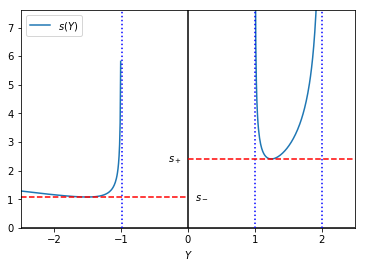
\includegraphics[width=.7\textwidth]{Images/s+s-.png}
\caption{Graphe de la fonction s(Y) et points d’intérêt.}
\end{figure}
On cherche le plus petit $s$, noté $s_{sel}$ tel que la condition d'amortissement sur $A$ soit vérifiée.\\
Pour $s> \max(s_+,s_-)$, $A$ a 4 racines réelles donc la condition d'amortissement est vérifiée.\\
Pour $s< \min(s_+,s_-)$, $A$ n'a pas de racines réelles donc la condition d'amortissement est violée.\\
Ainsi, $ \min(s_+,s_-) \leq s_{sel} \leq \max(s_+,s_-)$.
On va montrer que l'on a toujours $s_{sel} = s_-$: 
\begin{theorem}\textbf{{La plus petite vitesse en valeur absolue pour laquelle la condition d'amortissement est vérifiée correspond à la plus petite racine de $Q$, i.e. $s_{sel}=s_-$}}\\
Soit $s_{sel} =\min \{s>0,\text{Le polynôme $A_s$ vérifie la condition d'amortissement} \}$, i.e. la racines de plus petite partie réelle du polynôme $A_s= Y^4 + \frac{s^2}{T}P_3(Y)$ est réelle.\\
Soit $Q = 4P_3(Y)-YP'_3(Y)$ et soit $y_{min}$ sa plus petite racine (donc négative). Soit $s_- =  \sqrt{\frac{Ty_i^4}{P_3(y_i)}} $.
Alors \boxed{s_- = s_{sel}}
\end{theorem}
\begin{proof} \ \\
On a $ \min(s_+,s_-) \leq s_{sel} \leq \max(s_+,s_-)$.\\
La preuve se fait en deux cas:

\textbf{i) Premier cas:} $s_- < s_+$:\\
Dans ce cas, on sait déjà que $s_{sel} \geq s_-$ .\\
On va alors montrer que $A_{s_-} = Y^4+ \frac{s_-^2}{T}P_3(Y)$, ce qui donnera $s_{sel} \leq s_-$ donc $s_{sel} = s_-$.\\
Soit $Y_{1}$ la plus petite racine de $Q$. Nécessairement, $A_{s_-}$ a une racine double en $Y_1$. \\
Soit alors $Y_2$ et $Y_{3}$ ses deux autres racines. \\
Comme $s_-<s_+$, $Y_2$ et $Y_3$ sont des racines complexe conjuguées.\\ Grace aux relations de Viète (relations coefficients racines), on a:\\
\begin{equation}
	2Y_1 + 2\Re(Y_2) = - \frac{s_-^2}{T}(\lambda + f_0)	
\end{equation}
donc \begin{equation}
	2\Re(Y_2) =  - \frac{s_-^2}{T}(\lambda + f_0)	- 2Y_1.
\end{equation}
Or \begin{equation}
	\frac{s_-^2}{T} = \frac{Y_1^4}{P_3(Y_1)}
\end{equation}  
donc: \begin{align*}
	2\Re(Y_2) &=  - \frac{Y_1^4}{P_3(Y_1)}(\lambda + f_0)	- 2Y_1 \\
	&=- \frac{Y_1}{P_3(Y_1)}((\lambda + f_0)Y_1^3 - 2P_3(Y_1))\\
	&=-\frac{Y_1}{P_3(Y_1)}(Q(Y_1)+F_0f_0(\lambda+2f_0)Y_1 - 2F_0^2f_0^2)
\end{align*}
or $Q(Y_1) = 0$ et $Y_1<0$ et $P_3(Y_1)<0$ donc: \begin{equation}
	\Re(Y_2)>0.
\end{equation}
En particulier $Y_1 < \Re(Y_2)$ donc la racine de plus petite partie réelle est réelle donc $A_{s_-}$ satisfait la condition d'amortissement. Ainsi dans ce cas, \underline{$s_{sel} = s_-$}.\\

\textbf{ii) Deuxième cas:} $s_- > s_+$:\\
Dans ce cas, on sait déjà que $s_{sel} \leq s_{-}$.\\
On va alors montrer que $s_{sel} \geq s_{-}$. Pour cela, on va prendre $s \in [s_{+},s_-[$ et montrer que $A_s$ ne satisfait pas la condition d'amortissement.\\
Soit $s\in [s_{+},s[$.\\
 $A_s$ a deux racines réelles positives $Y_3$ et $Y_4$ et deux racines imaginaires conjuguées $Y_1$ et $Y_2$. \\ 
Montrons que $\Re(Y_1)<0$, ce qui montrera que la racine de plus petite partie réelle est imaginaire et donc $s_{sel} \not = s$.\\
Grace aux relations de Viète (relations coefficients racines), on a:\\
\begin{equation}
	2\Re(Y_1)  =  -Y_3 - Y_4 - \frac{s^2}{T}(\lambda + f_0)	 <0
\end{equation}
Ainsi, $\Re(Y_1)<0<Y_3,Y_4$ et donc $s_{sel} \not = s \ \forall s \in [s_{+},s_-[$. Or $s_sel \in [s_{+},s_-]$ donc \underline{$s_{sel} = s_-$}.\\
\ \\
Ainsi dans nos deux cas, on a \underline{$s_{sel} = s_-$}.

\end{proof}
\ifdefined\COMPLETE
\else
\end{document}
\begin{algorithm}[H]
\SetAlgoLined
\KwResult{Vitesse d'onde extrémale $s$ de l’équation d'onde associée au fluide}
 Entrées: données $\lambda$, $f_0$, $F_0$, $T$ et un $\epsilon$ choisi petit\;
 Calculer les racines réelles $y_i$ du polynôme $Q$ défini par \ref{eq:Q}\; 
 Candidats = $[]$\;
 \For{$y_i$ racine réelle de $Q$}{\If{$P_3(y_i)<0$}{Poser $s_i^2 = -\frac{y_i^4}{P_3(Y_i)}$ avec $s_i<0$\;
 Candidats $+=$ [$s_i$]}
 {}}
 \For{$s_i \in$ Candidats}{\If{le polynôme $Y^4 +(s_i^2-\epsilon)P_3(Y)$ n'a pas 4 racines réelles}{Candidats = Candidats \textbackslash $\{s_i\}$}}
 $s= \max$(Candidats)
 \caption{Recherche de la vitesse d'onde pour l’équation fluide}
\end{algorithm}
\fi

